%File: formatting-instruction.tex
\documentclass[letterpaper]{article}
\usepackage{aaai}
\usepackage{times}
\usepackage{helvet}
\usepackage{courier}
\usepackage{url}
\usepackage[pdftex]{graphicx}
\usepackage{amsmath}
\usepackage{latexsym}
\usepackage{amssymb}
\usepackage{multirow}
\newtheorem{definition}{Definition}
\frenchspacing
\setlength{\pdfpagewidth}{8.5in}
\setlength{\pdfpageheight}{11in}
\pdfinfo{
/Title (From Topics to Opinions: Modelling Subjectivity for Retweeting Analysis on Twitter)
/Author (Songxian Xie, Jintao Tang, Ting Wang, Ruili Wang, Kewen Wang)}
\setcounter{secnumdepth}{0}  
 \begin{document}
% The file aaai.sty is the style file for AAAI Press 
% proceedings, working notes, and technical reports.
%
\title{From Topics to Opinions: \\Modelling Subjectivity for Retweeting Analysis on Twitter}
%\author{Songxian Xie, Jintao Tang \and Ting Wang\\
%School of Computer, National University of Defense Technology, Changsha, P.R. China\\
%\AND Ruili Wang\\
%School of Engineering and Advanced Technology, Massey University, Auckland, New Zealand\\
%\AND Kewen Wang\\
%School of Information and Communication Technology, Griffith University, Brisbane, QLD 4111 Australia\\
%}
\nocopyright
\maketitle
\begin{abstract}
\begin{quote}
In this paper, we investigate how user's subjectivity influence their information diffusion behavior. 
Inspired by psychological research, we define a general subjectivity model by combining both topics and opinions articulated in User-Generated Content (UGC) and propose an efficient framework to establish the subjectivity model. 
We also put forward a new way to measure the subjectivity similarity between two subjectivity models. For the retweeting behavior analysis, three factors (attractiveness, sociality and popularity) are considered based on the subjectivity similarities among a target tweet, its author and followers. In the experiments, we demonstrate that a user is more likely to retweet a message considering the influence of the three factors and the utility of our model in retweeting analysis is verified qualitatively and quantitatively on real Twitter dataset.
\end{quote}
\end{abstract}

\section{Introduction}
\label{introduction}
\noindent Information diffusion has drawn considerable research attentions from computer scientists, especially in the area of online social networks. Researchers have built standard models for the general information diffusion,  which are useful for simulating the information flow\cite{goldenberg2001talk,kempe2003maximizing}, or detecting the outbreak of information cascades\cite{cheng2014can}. In this work, we target at a different problem: given a new message, we intend to predict which users will participate in the future diffusion process of this messsage\cite{Bian2014}. 
An illustration of the problem in a heterogeneous social network of Twitter can be found in Figure~\ref{fig00}. 
\begin{figure}[htb]
\centering
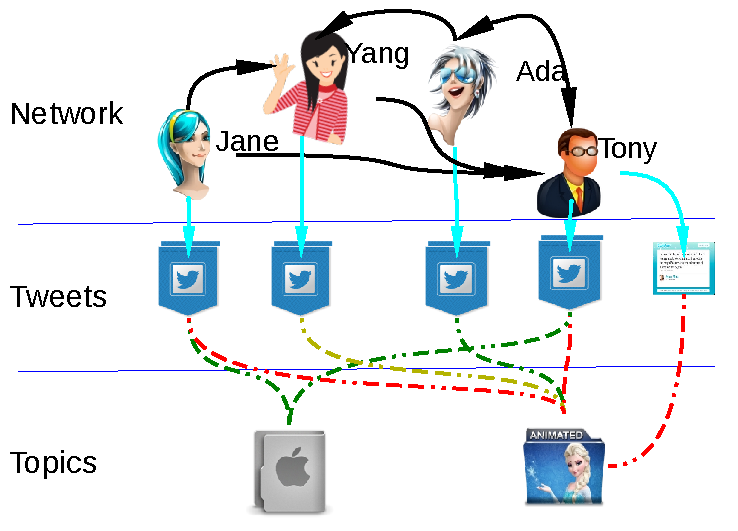
\includegraphics[width=2.2in,height=1.5in]{Mexample.pdf}
\caption{Motivating example. For opinions of different users, the color ``red'' stands for positive evaluation, ``green'' for negative, and ``yellow'' for neutral.}
\label{fig00}
\end{figure}
In this example, the users have tweeted about two topics: cellphone ``Iphone'' and movie ``Frozen''. Now Tony posts a new tweet about movie ``Frozen'', we want to find out which one is more likely to disseminate it among all the receivers of the new tweet.

As the participants of information diffusion, humans naturally make communication and interaction by expressing opinions and preferences about the topics that interests them. In psychology, it has been identified that the subjective initiative nature of human determines that subjectivity will undoubtedly influence human's behaviors \cite{moore2008awareness}. According to theory of Biased Assimilation, people tend to choose and disseminate information according to their own biased opinions \cite{Hyman2000}. Therefore, opinion and sentiment comprehension are a key aspect of users interaction in the process of information diffusion. 

The propagation behaviors are different in different social networks. Twitter plays an important role in the process of information dissemination on the Internet because the retweeting convention provides an unprecedented mechanism for the spread of information despite the restricted length of a single message. 
Actually almost a quarter of the tweets are retweeted from others \cite{yang2010understanding}. 
Understanding how retweeting behavior works can help explaining information diffusion on Twitter. 

Previous studies have developed a variety of techniques and models to capture the factors of retweeting behaviors \cite{macskassy2011people,feng2013retweet}. However few studies have investigated the subjective motivation of a user to retweet a message. 
From the point of a user, retweeting is a process that includes following, evaluating and deciding whether to share. The crucial part is to evaluate whether a tweet contains information worthy enough to be shared.  
Therefore modelling the subjective motivation of users will provide an important perspective for retweeting behavior analysis. 
Intuitively, based on the principle of ``like attracts like'', a biased user is more prone to retweet a message that meets his own tastes. In Figure~\ref{fig00}, the tweets of the users present their different opinions about two topics. Tony and Jane were positive about movie ``Frozen'', while Ada was negative and Yang was neutral. For the new tweet of Tony which is positive about ``Frozen'', Jane is more likely to retweet it because they both like the movie. 

For the problem to be investigated, there are two questions arising: how to accurately model the subjectivity of users in terms of topics and opinions, and how to effectively measure the worthiness for the users to retweet? 
Answering the questions is non-trivial. 
In this paper, we propose a general method to model subjectivity of users, define a novel similarity measurement to calculate the worthiness,  and identify factors that influence a user's retweeting behavior considering his subjectivity. 

The rest of the paper is organized as follows: firstly related works are described; we give the definition and establishment details of the proposed subjectivity model, before the subjectivity similarity is defined; then the factors are specified for the retweeting analysis problem;following are experiments of quantitative evaluation; and we summarizes the paper and points out future work finally.

\section{Related Work}
\label{relatedwork}
   
A large body of studies have analyzed characteristics of retweeting behavior \cite{Bian2014,Luo:2013RMF}, examining factors that lead to increased retweetability \cite{suh2010want,comarela2012understanding} and designing models to estimate the probability of being retweeted \cite{jenders2013analyzing,pfitzner2012emotional}. However, all of the above works neglect the subjectivity of users, which is the underlying reason for the retweeting behaviors. 

Previous researches of sentiment analysis have mainly focused on reviews \cite{liu2012sentiment}. 
Recently, there have been many works on sentiment analysis for informal social media langage, mainly focusing on the message level \cite{jiang2011target,tan2011user,Guerra2014}. Topic models can also be utilized in sentiment analysis to correlate sentiment with topics. For example, Mei \emph{et al.}~\cite{mei2007topic} and Lin \emph{et al.}~\cite{lin2009joint} attempted to incorporate the sentiment factor into topic models. Usually they learn a general word-sentiment distribution to model the sentiment of blogs or reviews, which may not work well for short and informal social media languages. Sentiment expression is deemed to be more challenging as sentiment is often embodied in subtle linguistic mechanisms such as: negation, capitalization, repeated letters, exclamation and emoticon(e.g. ``happy!!''), intensifiers (e.g. ``liked'' versus ``liked verymuch'') and diminishers (e.g. ``excellent'' versus ``rather excellent''),etc \cite{brody2011col}. These are hard to be modeled with probabilistic distribution. However, rule-based sentiment analysis methods can catch such subtle sentiment expressions by transforming the them into rules \cite{thelwall2010sentiment}. In our model establishment framework, we adopt rule-based method for tweet sentiment analysis.

\section{Subjectivity Model}
\label{subjectivemodel}

Subjectivity has been extensively studied by psychologists to characterize the personality of a person based on his historical behaviors and remarks \cite{engbert2007agency}. 
Linguists define the subjectivity of language as speakers always show their perspectives, attitudes and sentiments to events, people, topics, and entities in their linguistic contents \cite{stein2005subjectivity}. In the computer sicience, opinion mining techniques \cite{liu2012sentiment} have been developed to computationally model the subjectivity of users. With the explosion of social media over the past decade, more and more User-Generated Content (UGC) is available on the Web for expressing users' opinions. A variety of aspect-level and topic-sentiment models have been built from UGC by casting opinions as polarity, strength, or emotions regarding a topic \cite{lek2013aspect,mei2007topic}. We give a general framework to model subjectivity by combining topics and opinions together. Here we give our definition of subjective model under context of Twitter, while we emphasize that our model can be transfered to other data platforms as well.

\subsection{Definition}
\label{definition}

Let $G=\left( V,E \right) $ denote a social network on Twitter, where $ V $ is a set of users, and $ E\subset V\times V $ is a set of follow relationships between users. For each user $ u \in V $, there is a tweets collection $ M_{u} $ denoting his message history. We assume that there is a topic space $ T $ containing all topics users in $ V $ talk about, and a sentiment space $ S $ to evaluate their opinions towards these topics. 
For the ``subjectivity'' of a user $ u  \in V $, we refer to both topics and opinions articulated in his tweets collection $ M_{u} $.  
\begin{definition}[Subjectivity Model]
The subjectivity model of user $ u $, is the combination of topics of interest $\left\lbrace  k \right\rbrace $ in topic space $T$ and his opinions $\left\lbrace O_{k}\right\rbrace $ towards each topic distributed over sentiment space $ S $. 
\begin{equation}
\label{usermodel}
SM_{u}  = \lbrace \left( k, w_{u,k} , \lbrace d_{u,k,s} |s \in S \rbrace \right) |  k \in T \rbrace
\end{equation}
where:
\begin{itemize}
\item with respect to user $ u $, for each topic $k \in T$, its weight $ w_{u,k} $ represents the distribution of the user's interests on it, subject to $ \sum_{t=1}^{|T|}w_{u,k} =1 $.
\item opinion of the user towards topic $t$ is modelled as a topic-dependent sentiment distribution over sentiment space $ S $, $O_{k}=\lbrace d_{u,k,s}|s \in S \rbrace $, subject to $ \sum_{s=1}^{|S|} d_{u,k,s}=1$.
\end{itemize}
\end{definition}
Our model is more general than others in that we combine the topics of interest and topic-dependent opinions into a holistic framework, and more importantly, we define opinion as a probabilistic distribution in a scalable sentiment space. The sentiment space can cover all the sentiment modalities, for example, it could be binary value standing for positive and negative polarity, or sequential value for sentiment strength, or discrete value for various emotions. 
Figure~\ref{fig0} is a visualized subjectivity model example in a $ [0,100] $ topic space and a discrete $ [0,8] $ sentiment space. 
\begin{figure}[t]
%\centering
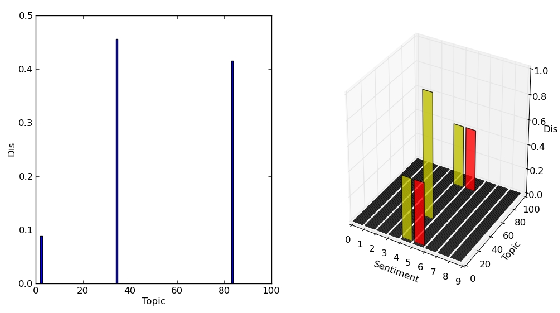
\includegraphics[width=3.3in,height=1.2in]{fig1.pdf}
\caption{Subjectivity model example. The left subgraph denotes interests distribution on topic 2, 32 and 83: $ (  w_{u,2}=0.08,w_{u,32}=0.48, w_{u,83}=0.44)  $. The right subgraph denotes opinions towards topics: $ O_{2}=( d_{u,2,4} =0.5, d_{u,2,5} =0.5)$, $O_{32}=(d_{u,32,4}=1.0) $, $ O_{83}=( d_{u,83,4}=0.5, d_{u,83,5}=0.5 ) $.}
\label{fig0}
\end{figure}
The definition of the subjectivity model is in an abstract form, which needs to be concreted from two aspect:(1)how to construct the subjectivity model (2)how to utilize this model for retweeting analysis.
 
\subsection{Establishment of Subjectivity Model}
\label{establishment}

In this section, we present our method to construct subjectivity model $ SM_{u }$ by deriving topics and opinions from the message histories of all users $ M=\lbrace M_{u}\vert u \in V\rbrace$.

\subsubsection{Topic Analysis}
\label{topic}

In this paper, we simply use the concept of topics to broadly refer to the different kinds of content such as bag-of-words, entities, hashtag, etc. Previous studies have tried to identify topics from tweets by finding key words \cite{chen2010short}, extracting  entities \cite{abel2011analyzing} or linking tweets to external knowledge categories \cite{macskassy2011people}. However, works show that topic model is more effective in identifying topics from short and informal social media language \cite{hong2010empirical}. State-of-the-art topic model such as Latent Dirichlet Allocation (LDA) \cite{blei2003latent} is employed for unsupervised topic discovery and for topic assignment of future documents. LDA can be used to find a set of $ K $ latent topics from a document corpus, and then to represent each document $ D $ with a distribution $ \theta_{D} $ of the latent topics. For each word $ w_{i} $ in $ D $, a topic $ z $ is first sampled from the document topic distribution $ \theta_{D} $, then $ w_{i} $ is sampled according to word distribution $ \phi_{z} $ of topic $ z $. 

As the first step, we adopt the user-level LDA model to build a global Topic Model (TM), which regards all tweets of a user as one document of LDA \cite{hong2010empirical}. The TM model will be used throughout our framework. For a single tweet $ t $, each dimension $ i $ of its topic distribution $ \theta_{t} $ can be obtained as follows:
\begin{equation}
\theta_{t,i}=\dfrac{\prod_{w \in t}P(w|\phi_{i})}{\prod_{w \in t}\sum_{k}P(w|\phi_{k})}
\end{equation}
Usually a tweet concentrates a single topic within its short length, therefore we assign a tweet $ t $ to a topic that maximizes the probability of generating $ t $:
\begin{equation}
\label{twtopic}
z_{t} = \arg \max_{k}\prod_{w \in t} P(w|\phi_{k})
\end{equation}
Finally we can get the weight distribution on each topic $ k $ of user $ u $ by normalizing all tweets that talk about topic $ k $: 
\begin{equation}
w_{u,k}=\dfrac{|\{ t: t \in M_{u} \wedge z_{t}=k\}|}{|M_{u}|}
\end{equation}

\subsubsection{Opinion Analysis}
\label{opinion}

Most previous opinion mining researches \cite{liu2012sentiment} represent opinion with a porlarity label in a binary sentiment space (0, 1): 1 means opinion agreement or positive sentiment, 0 means opinion disagreement or negative sentiment. However, such approach cannot fully distinguish user's detail opinion. For example, in Figure~\ref{fig00}, both Tony and Jane holded overall positive opinion about the movie ``Frozen''. Jane mainly liked the romantic story of this movie but was a little disappointed about its animation picture, while Tony liked this movie because he was mostly convinced by its animation technology although he disliked the prince and princess genre. If we represent their opinions with a simple binary polarity manner, without differentiating their preferences of different aspects, the subjectivity model may not satisfy the information discovery needs of different users. Therefore,considering different aspects of a topic, it is better to describe opinion for a topic as a probability distribution over the sentiment space. Furthermore, a more fine-grained sentiment space is preferred if we want to distinguish subjectivities of users more precisely.

Researches on the sentiment analysis of social media have provided many effective state-of-the-art techniques and tools \cite{thelwall2010sentiment,hu2013unsupervised}, with which sentiment of a tweet $ t $ can be identified as $ s_t $. The opinion distribution $ O_k $ toward a topic $ k $ is got as:
\begin{eqnarray}
O_k &= & \{ d_{u,k,s}|s \in S \}\\
  &=& \{ \dfrac{|t:t \in M_u \wedge z_t=k \wedge s_t=s|}{|M_u|}|s \in S\}
\end{eqnarray}

\subsection{Subjectivity Similarity}
\label{similarity}

With the subjectivity models estabilshed, the subjectivity similarity needs to be defined and calculated to simulate the various subjective decision-making process such as retweeting behavior. 
In this section, we define a novel similarity measurement to quantify the subjectivity similarity. 
 
\subsubsection{Opinion Similarity}
\label{opsim}

Opinion in the subjectivity model is treated  as a distribution over sentiment space with each dimension of the distribution representing the proportion of the corresponding sentiment value. 
At the same time, values in the sentiment space are not independent. 
They are sequential in magnitude and quantified to measure the strength of sentiment. Therefore, normal distrbution similarity measurements such as KL-divergence and consine similarity are not suitable for such kind of opinion distribution. For example,illustrated in Table~\ref{tab1}, in a $ [0,8 ] $ integer sentiment space, opinion $ O_{k}^{1} $ is most negative (100\% of value 0), opinion $ O_{k}^{2} $ (100\% of value 6) is positive, and $ O_{k}^{3} $ (100\% of value 8) is most positive.
If the cosine similarity measurement is adopted to calculate opinion similarity, all similarities among them are 0.
In fact $ O_{k}^{2} $ is more similar with $ O_{k}^{3} $ than $O_{k}^{1} $ because they both hold positive opinion and their sentiment strength distance is much less than with $ O_{k}^{1} $.  
Therefore, opinion similarity can't be calculated simply as the normal probabilistic distributions, or just as the sentiment strength distance. 
To accurately catch opinion similarity, we propose a novel method by combining both sentiment distance and distribution similarity.
The opinion similarity between two opinions $O_{k}^{1},O_{k}^{2} $on the same topic $ k $ can be calculated as: 
\begin{equation}
\label{opinionsim}
Sim(O_{k}^{1},O_{k}^{2})=\dfrac{|S|-|\sum_{i=0}^{|S|}d_{i}^{1}v_{i}-\sum_{i=0}^{|S|}d_{i}^{2}v_{i}|}{|S|}
\end{equation}
where $ d_{i} $ denotes the $ i^{th} $ dimension of opinion distribution, and $ v_{i} $ denotes corresponding sentiment strength value. 
\begin{table}[htb]
\scriptsize
\centering
\caption{Illustration of opinion similarity}
\label{tab1}
\begin{tabular}{|l|l|l|l|l|l|l|l|l|l|}
\hline
 & 0 & 1& 2 & 3 & 4 & 5 & 6 & 7 & 8 \\
\hline
$O_{t}^{1}$ & 1.0 & 0.0 & 0.0 & 0.0 & 0.0 & 0.0 & 0.0 & 0.0 & 0.0 \\
\hline
$O_{t}^{2}$ & 0.0 & 0.0 & 0.0 & 0.0 & 0.0 & 0.0 & 1.0 & 0.0 & 0.0 \\
\hline
$O_{t}^{3}$ & 0.0 & 0.0 & 0.0 & 0.0 & 0.0 & 0.0 & 0.0 & 0.0 & 1.0 \\
\hline
\end{tabular}
\end{table} 
The similarities of opinions in Table~\ref{tab1} calculated with Equation~\ref{opinionsim} are $ Sim(O_{k}^{1},O_{k}^{3})=0 $, $ Sim(O_{k}^{2},O_{k}^{3})=6/8 $ and $ Sim(O_{k}^{1},O_{k}^{2})=1/8 $, which are consistent with our intuitive understanding. 

\subsubsection{Subjectivity Similarity}

As the subjectivity model indicates, a user may be interested in several topics and the weights of interests is a distribution over topic space $ T $.Therefore, the subjectivity similarity between two subectivity models should be integrated from the distribution of topics of interest and the opinion similarities on each topic. Accordingly, overall sbjectivity similarity between two subjectivity models $ SM_{u},SM_{v} $ can be calculated as: 
\begin{equation}
\label{subsim}
Sim(SM_{u},SM_{v})=\dfrac{\sum_{k=1}^{|T_{u,v}|}\theta_{u}(k)\* Sim(O_{k}^{u},O_{u}^{v})}{\sum_{k=1}^{|T_{u,v}|}\theta_{u}(k)}
\end{equation}
where $ T_{u,v} $ denotes the common topics between two users $ u $ and $ v $, which can be regarded as the intersection between their topics of interest with $ \theta_u^k\neq 0\wedge \theta_v^k\neq 0$; $ \theta_{u}(k) $ denotes the topic $ k $ weight of user $ u $, and $ \sum_{k=1}^{|T_{u,v}|}\theta_{u}(k) $ is the normalized factor.

Note that, the subjectivity similarity is asymmetric because when we measure how similar user $ u $ is with user $ v $ we use the weights of common interests of user $ u $. The intuition lies in that subjectivity of a user is a personal inner interest and taste, and it is also a subjective decision to judge a like-minded person for the user. For our measurement of subjectivity similarity, $ Sim(SM_u,SM_v)\neq Sim(SM_u,SM_v)$.

\section{Retweeting Analysis}

Whether a user propagate a tweet may be affected by various factors. From the point of a user, a tweet is more likely to be retweeted because the user finds its content worth to. Generally three factors need to be considered: 1) the content of the tweet is in accordance with a user's subjectivity, which are attractive for the user to retweet; 2) the tweet is posted by the user's like-minded close friend, and his retweeting behavior is due to social needs; and 3) the content is novel or epidemic, and his retweeting behavior is a result of conformity needs (i.e., the act of matching opinions to group norms \cite{cialdini2004social}). In this section, we firstly formulate the retweeting analysis as a classfication problem, then present the analysis of the three factors considering subjectivity for understanding the underlying reasons that a user disseminates the tweet based on his subjective initiative. 

\subsection{Problem Formulation}
\label{formulation}

For a target tweet $ m $, let $ F $ denote the followers who receive $ m $ by following its author $ u_{a} $, and for each user $ u \in F \cup \left\lbrace u_{a} \right\rbrace  $, let $ M_{u} $ denote a tweet collection $ u $ has published. 
For each follower $ f \in F $, we can define a quadruple $ <f, u_{a}, m, r_{f}>  $: 
\begin{itemize}
\item $ r_{f} $ is a binary label indicating if $ m $ is retweeted by $ u $, which should be predicted for a future tweet.
\item Firstly our work focuses on building subjectivity model $ P\left( u \right)  $ for each user $ u \in F \cup \left\lbrace u_{a} \right\rbrace $ with all tweets collections $ M=\left\lbrace M_{u} | u \in F \cup \left\lbrace u_{a} \right\rbrace  \right\rbrace  $.
\item Then we investigate the relation between the subjectivity of a user and his retweeting behavior to predict $ r_{f} $ by calculating subjectivity similarities between tweet $ m $, its author $ u_{a} $ and follower $ u $. 
\end{itemize}

\subsection{Retweeting Analysis}
\label{analysis}

The three factors exhibit different types of reasons a user rewteet a microblog, which will be analyzed and quantized in this section.

\subsubsection{Attractiveness}

A user is likely to repost a microblog if the user finds the content is attractive according to his subjective judgement. We can measure such attractiveness quantitatively by calculating the subjectivity similarity between the tweet $ t $ and user $ f $. For a tweet $ t $, its topic $ z_t $ can be identified with Equation~\ref{twtopic}, and let $ s_t $ be its sentiment. The content of $ t $ can also be modeled using our subjectivity model definition with a single topic of interest and a \%100 opinion distribution on a single sentiment value. Thus the attractiveness of the tweet can be measured with subjectivity similarity using Equation~\ref{subsim}, which is marked as $ Sim(f,t) $.

\subsubsection{Sociality}

In this case, the retweeting behavior is based on the needs of social interaction. That is, the behavior is triggered because the tweet $ t $ is sent by a like-minded friend, instead of the information it contains. We can measure how like-minded the user $ f $ and his friend $ u_a $ with their subjectivity similarity $ Sim(f,u_a) $.  However, different kinds of friends may have a different influence on the user $ f $. For example, $ f $ may follow many friends, but only frequently interacts with a few. Furthermore, not all tweets of a friend may be of interest to $ f $. For example, in Figure~\ref{fig00}, Jane may be interested in tweets from Tony about movie, but may not be interested in his tweets about cellphone. We therefore assign a weight to $ Sim(f,u_a) $ to reflect the influence of different kinds of friend, which
is composed of four factors:\\
\emph{Expert Factor $ w_E(u_a) $}: it calculates the relative expertise of the tweet author among his followers including $ f $. The expert user impose more influence on others than the others do. We simply calculate it as the ratio of user $ u_a $'s tweets count over all tweets of $ u_a $ and his followers by $ w_E(u_a)=|M_{u_a}|/|\{M_u|u \in u_a \cup F \}|  $.\\
\emph{Leadership Factor $ w_L(u_a) $}: In our work, the leadership of a user $ u_a $ is determined by his followers. The leadership weight is calculated by $ w_L(u_a)=\log (|F|)/\log(\max) $, where $ \max $ is the maximum popularity of a user in Twitter\footnote{\url{http://twittercounter.com/pages/100}}.\\
\emph{Similarity Factor $ w_S(u_a,f) $}: The similarity of interests of $ u_a $ and $ f $ is measured as the inverse KL-divergence between their topic distribution in their subjectivity model: $ w_S(u_a,f)= 1/KL(\theta_{u_a},\theta_f)$.
\emph{Interaction Factor $ w_I(u_a,f) $}: All the interactions $ Interation_{u_a,f} $ between $ u_a $ and $ f $ are analyzed, which include the conversations between them, mentions of each other, and retweets from each other. The factor weight is calculated by normalizing $Interation_{u_a,f}$ with all tweets of $ u_a $ and $ f $: $ w_I(u_a,f)=|Interation_{u_a,f}| /|\{ M_{u_a}, M_f \}| $.\\
Above all, the influence weight is the combination of four factors:
\begin{equation}
\begin{split}
w_{u_a,f}=\lambda_1*w_E(u_a)+\lambda_2*w_L(u_a)+\lambda_3*w_S(u_a,f)\\+\lambda_4*w_I(u_a,f). 
\end{split}
\end{equation}
where $ \lambda_i $ is an optional weight vector to enable different influence of the factors,  subject to $ \sum_{i=1}^{4}\lambda_i=1 $.

\subsubsection{Popularity}

If a tweet is popular (e.g., breaking news), it will be very probable to be retweeted. In this situation, the tweet $ t $ is often inconsistent with the interests and opinion of its author $ u_a $. Thus the similarity between $ t $ and $ u_a $ in terms of subjectivity is very low, which is marked as $ Sim(u_a,t) $. The retweeting behavior is highly related to the popularity of $ t $ rather than the content or the friend who post it. We assign a popularity weight $ w_P $ to $ Sim(u_a,t) $, which is the proportion of user $ f $'s followees who have retweeted the tweet $ t $.

From the point of motivation, a user might retweet a message if its content is approximate to his subjectivity, its author is a like-minded friend and it is popular among his friends. 
In next section we carry out a set of experiments to inspect and verify the impact of such motivation on retweeting behavior. 

\section{Experiments}
\label{experiments}

\subsection{Dataset and Settings}
We adopt the Twitter dataset of a previous work \cite{Luo:2013RMF}. 
To form the dataset, 500 target English tweets published from September 14th, 2012 to October 1st, 2012 were monitored to find who would retweet it in the next days. 
Besides, each target tweet was set as starting point to collect at least 200 historical tweets for its author and followers.
Overall, there are 45,531 users who have posted at least 6,277,736 historical tweets, 5214 of which retweet at least one target tweet during the monitored period. To avoid the bias introduced by dataset imbalance, an evaluation dataset was constructed by taking 5,214 retweeters as positive instances, and randomly sampling 5,214 non-retweeters as negative instances. 

For the topic model of LDA, we use variational inference-based topic model package Gensim \cite{rehurek_lrec}, which adopts an efficient batch-based online inference algorithm and can easily adapt to new document. All parameters are set as defaults and the number of topic traverses from 50 to 200. For sentiment analysis of each tweet, we just make use of an off-the-shelf work, i.e. SentiStrength \cite{thelwall2010sentiment}. In order to catch the sentiment of tweets, we use the sentiment lexicon created based on AFINN by Nielsen \cite{MohammadKZ2013}. The sentiment space is formed by mapping the positive and negative sentiment values to range $ [0,8] $.

\subsection{Correlation Test}

First of all we assess the correlation between subjectivity similarity and retweeting behavior with a statistical hypothesis test Analysis of Variance (ANOVA) \cite{fisher1970statistical}, which tests the \textit{null hypothesis} that whether the retweeters and non-retweeters have the same subjectivity similarity means. 
The results are listed in Table~\ref{tab2}. The bold-faced entries mean that the \textit{p-value} is lower than significance level.
\begin{table}[htb]
\scriptsize
\centering
\caption{ANOVA results for subjectivity similarities. If the difference is due to chance, \textit{F-ratio}=1.00, otherwise \textit{F-ratio} \textgreater 1.00 (\textit{p-value} \textless 0.01).}
\label{tab2}
\begin{tabular}{|c|c|c|c|c|}
\hline
\multicolumn{2}{|c|}{Similarity}& $ Sim(f,t) $ & $ Sim(f,u_a)  $ & $ Sim(u_a,t)  $\\
\hline
\multirow{2}{*}{50} & \textit{F} & \textbf{12.182} & 2.212 & 4.236 \\
\cline{2-5}
  & \textit{p} &  $\mathbf{4.44e^{-06}}$  & 0.140 & 0.272\\
\hline
\multirow{2}{*}{100} & \textit{F} & \textbf{43.892} & \textbf{31.145} & \textbf{28.466} \\
\cline{2-5}
  & \textit{p} &  $\mathbf{8.65e^{-11}}$  & $\mathbf{3.55e^{-08}}$ & $\mathbf{1.32e^{-09}}$\\
\hline
\multirow{2}{*}{150} & \textit{F} & \textbf{22.356} & \textbf{12.240} & \textbf{14.664} \\
\cline{2-5}
  & \textit{p} &  $\mathbf{2.43e^{-08}}$  & $\mathbf{6.25e^{-06}}$ & $\mathbf{8.46e^{-07}}$\\
\hline
\multirow{2}{*}{200} & \textit{F} & \textbf{31.675} & \textbf{20.616} & 6.145\\
\cline{2-5}
  & \textit{p} &  $\mathbf{4.22e^{-06}}$  & $\mathbf{2.92e^{-05}}$ & 0.26\\
\hline
\end{tabular}
\end{table}
Note that for the topic numbers of 100 and 150, all similarities yield \textit{p-values} below significance level with \textit{F-ratio} above 1.00. This suggests that the subjectivity similarities could be useful features for modeling retweeting behavior. 
For the rest experiments, we set the topic number as 100 for LDA model. 

\subsection{Case Study}
\label{example}
In this section, we give an vivid example to illustrate the subjectivity model and its ability in explaining the retweeting behavior. 
The subjectivity models of one of the 500 target tweets, its author, and two followers (one retweeter, the other non-retweeter) are shown as Figure~\ref{fig5}. 
The right part of each sub-figure illustrates topic distribution and the left part illustrates opinions towards each topic. 
\begin{figure*}[htb]
\centering
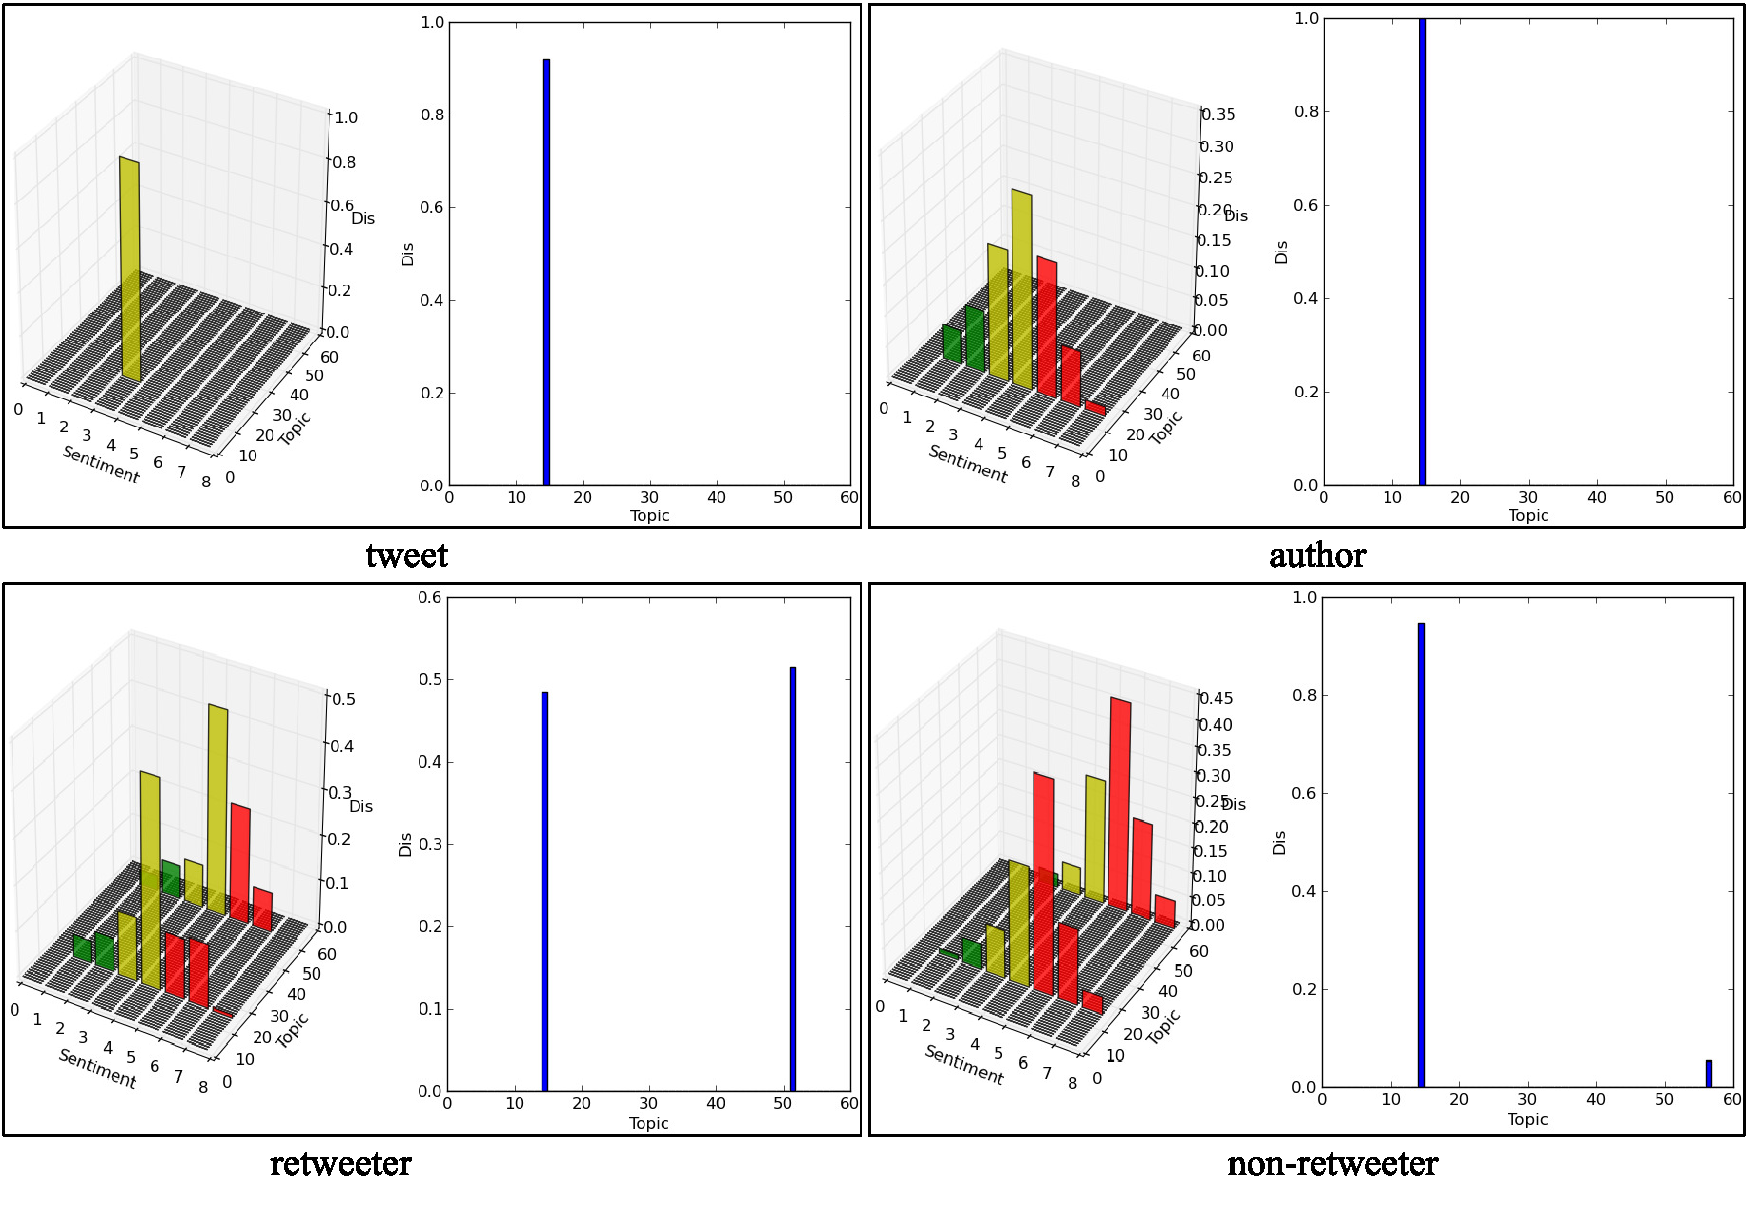
\includegraphics[width=5.5in,height=3.2in]{fig5.pdf}
\caption{An illustration of subjectivity models of a tweet, author and two followers.}
\label{fig5}
\end{figure*}
Figure~\ref{fig6} shows top words of the $ 14^{th} $ topic, the tweets of the author and two followers in word cloud diagrams\footnote{We use TagCrowd (\url{http://tagcrowd.com/}) to produce word cloud.}.
\begin{figure}[htb]
\centering
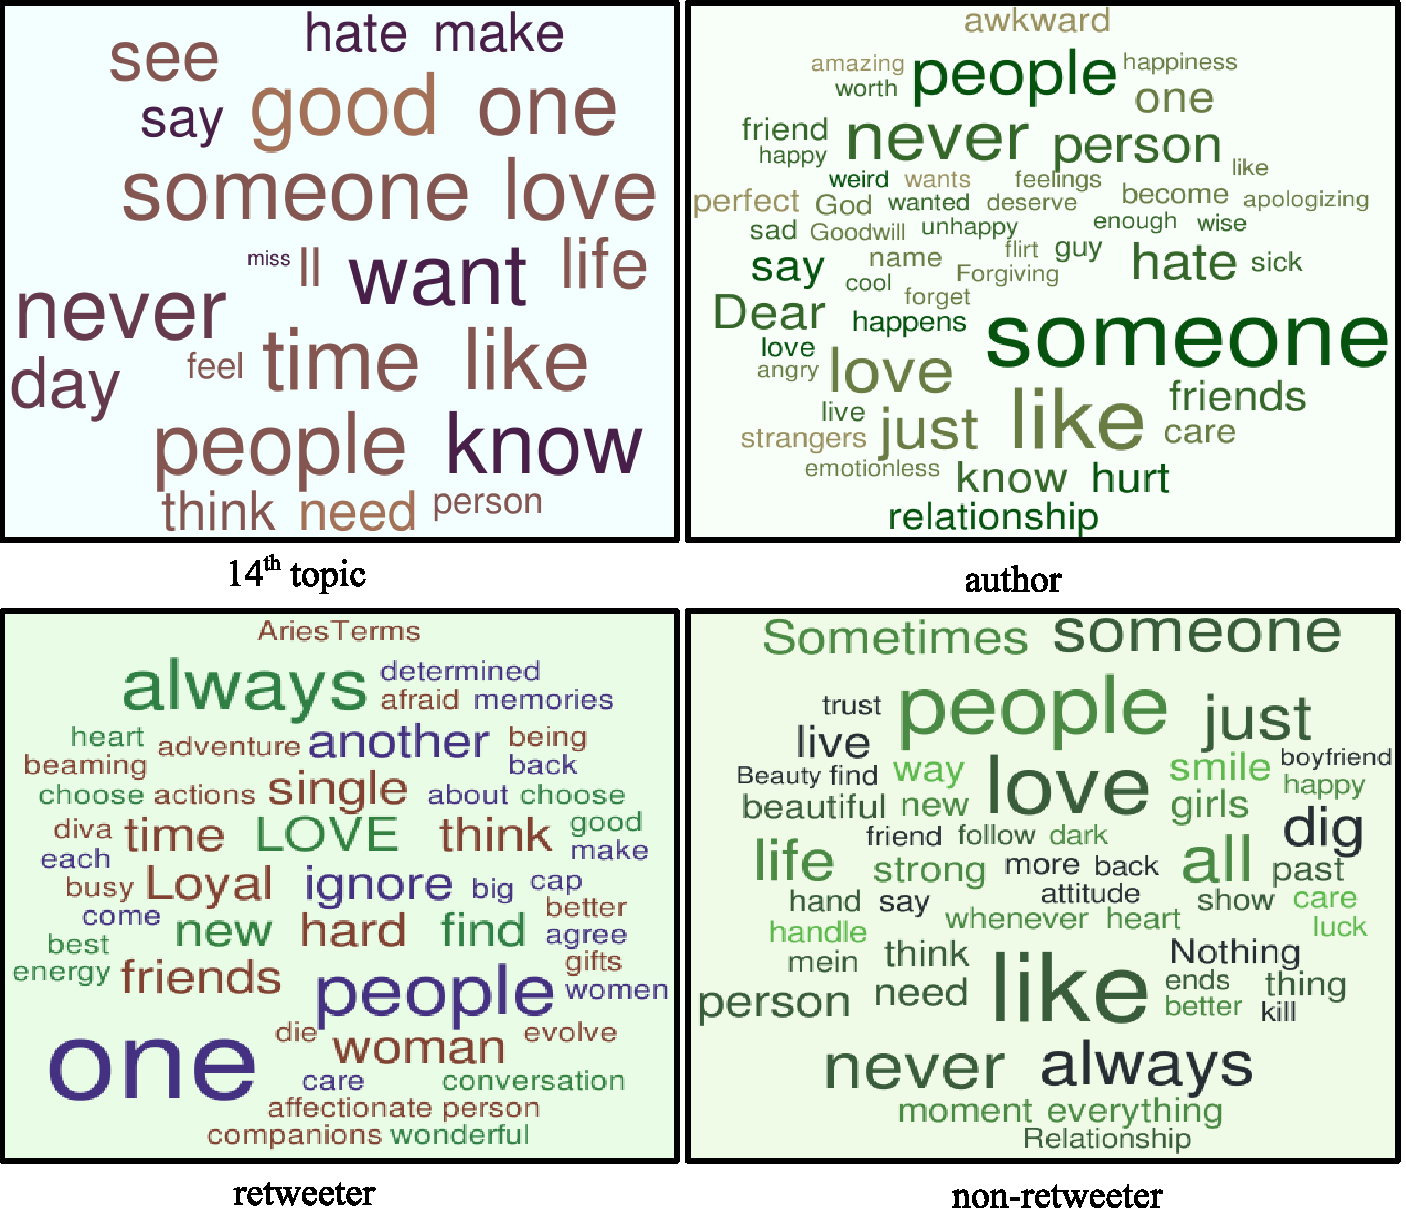
\includegraphics[width=3.2in,height=2.0in]{fig6.pdf}
\caption{Word cloud diagrams of the $ 14^{th} $ topic, author and followers.}
\label{fig6}
\end{figure}

The tweet is about the $ 14^{th} $ topic, and the opinion is neutral.
The author concentrates on the $ 14^{th} $ topic, and his opinion is mainly neutral.
% ($O_{u_{a}}^{14} =( 0, 0.04, 0.05, 0.25, 0.35, 0.25, 0.05,  0.01 )$). 
As for two followers, the retweeter has tweeted about two topics (the $ 14^{th} $ and $ 52^{nd} $ topic) uniformly 
%(with $ w_{u_{r}}(14)=0.48 $) 
and his opinion towards the $ 14^{th} $ topic is mainly neutral.
%($O_{u_{r}}^{14} =( 0, 0.02, 0.04, 0.15, 0.50, 0.13,  0.15,  0.01)$). 
While the non-retweeter has also talked about two topics ($ 14^{th} $ and $ 56^{th} $ topic), but he is mainly interested in the $ 14^{th} $ topic 
%(with $ w_{u_{n}}(14)=0.98 $) 
and his opinion is positive.
% ($O_{u_{n}}^{14} =( 0, 0.01, 0.04, 0.10, 0.25, 0.45, 0.13, 0.02)$).

Table~\ref{tab4} shows the three factors measurement for both retweeter and non-retweeter. 
\begin{table}[h]
\scriptsize
\centering
\caption{ Illustration of example subjectivity similarities}
\label{tab4}
\begin{tabular}{|c|c|c|c|}
\hline
Similarity & $ Sim(f,t) $ & $ Sim(f,u_a)  $ & $ Sim(u_a,t)  $\\
\hline
Retweeter & 0.854 & 0.967 & 0.886\\
\hline
Non-retweeter & 0.805 & 0.919 & 0.886\\
\hline
\end{tabular}
\end{table} 
Two followers have common interest (the $ 14^{th} $ topic), and furthermore the non-retweeter is more similar with the tweet and its author than the retweeter in terms of topics. But their different opinions towards the topic elicit their different behaviors, which verifies our model can help better understanding the retweeting behavior not only from topics but also opinions.

\subsection{Performance Evaluation}

We carray out the retweeting behavior prediction experiments with three stages. Firstly we compare our model against other topic-based models including TF-IDF model (modelling user interests with bag-of-words), entity-based model (modelling user interests with entities extracted from the UGC) and hashtag-based model (modelling user interests with hashtags used in the UGC)\cite{abel2011analyzing}. 

Secondly, our model is compared with two generative topic-sentiment models (TSM model \cite{mei2007topic} and JST model \cite{lin2009joint}). TSM and JST can also model topic and topic related sentiment simultaneously. We use Equation~\ref{subsim} for the subjectivity similarity of TSM and JST to get three factors values as our model.

Finally, our model tries to catch the subjective motivation of users based on UGC, whereas other important factors associated with retweeting behavior are not considered, such as network topology and characteristics of users. 
Therefore, our model is also compared with the method of Luo \emph{et al.}~\shortcite{Luo:2013RMF} (marked as ``LUO''), in which diffenent factors that might affect rewteeting behaviors have been considered.
In their work they use bag-of-words to model user interests, and we also carry out combining experiments to demonstrate that performance of prediction can be improved by replacing their bag-of-words model with our model (marks with ``LUO+'' prefix). 
\begin{table}[htb]
\scriptsize
\centering
\caption{Accuracy performance. A significant improvement over baseline with $ \ast $ and LUO's model with $ \ddagger $ ($p < 0.05$).}
\label{tab3}
\begin{tabular}{|l|l|l|l|}
\hline
Feature & Accuracy(\%) & Feature & Accuracy(\%)\\
\hline
baseline & 60.85 & & \\
\hline
TF-IDF & 62.85   $\ast$ & LUO & 71.76 $ \ast  $\\
entity & 68.76  $\ast$ & LUO+entity & 72.15 $\ast$\\
hashtag & 59.12  & LUO+hashtag & 68.44 $\ast$\\
\hline
TSM & 67.44 $\ast$ & LUO+TSM & 68.23 $\ast$\\
JST & 68.13 $\ast$ & LUO+JST & 70.53 $\ast$\\
\hline
$ Sim(f,t) $ & 73.88   $\ast  \quad \ddagger $ &LUO+$ Sim(f,t)$ & 74.04  $ \ast \quad \ddagger $\\
$ Sim(f,u_a)  $ & 70.04   $\ast  $ & LUO+$ Sim(f,u_a)$ & 70.27  $ \ast $\\
$ Sim(u_a,t)  $ & 69.64   $\ast  $ & LUO+$ Sim(u_a,t)$ & 71.86  $ \ast $\\
$ sim_{all}  $ & \textbf{75.64}   $\ast \quad \ddagger $ & LUO+$ sim_{all}  $ & \textbf{78.15}  $ \ast \quad \ddagger $\\
\hline
\end{tabular}
\end{table}

The logistic regression classifier is used for training and testing in a 5-fold cross-validation manner.
We set a baseline, which simply predicts users who have retweeted the author previously as the retweeters of target tweet. 
The classification results are presented in Table~\ref{tab3} in terms of accuracy.

Firstly, all models except the hashtag-based model outperform the baseline (60.85\%) significantly. While for hashtag-based model, its accuracy is only 59.12\%, the reason lies in the spacity of hashtag in tweets. 

Secondly, in the comparative results, $ Sim(f,t) $ and $ sim_{all}  $ outperform ``LUO'' (71.76\%) significatantly.
The best performance is achieved by the $ sim_{all}  $ (75.64\%), for which we add three factors values to the classifier to test the impact of their combination. 
The perfromance of TF-IDF model (62.85\%) is a little better than baseline. 
The entity-based model (68.76\%) is very close to  $ Sim(f,u_a)$ (70.04\%) and $ Sim(u_a,t)  $ (69.64\%), and the difference is not significant.

Thirdly, the performance of two topic-sentiment models (TSM: 67.44\%, JST: 68.13\%) is not as good as our models. The reason lies in that they use a binary sentiment representation (positive or negative), which can not differentiate opinions elaborately. Our model can capture more subtle and fine-grain sentiment strength, which could distinguish different subective motivation of retweeting behavior.

Finally, in the combining evaluation experiment, $ Sim(f,t) $ gives a significant improvement (LUO+$ Sim(f,t) $, 2.12\% improvement) over ``LUO'', but other two factors and the entity-based model can not improve performance significantly. The performance is even degraded after combining with the hashtag-based model and two topic-sentiment models. 
But noticing that, the most significant improvement(LUO+$ sim_{all}  $, 6.39\% improvement) is achieved by combining with all three factors. 

The results above show that subjectivity model can better help predicting retweeting behavior than other models and can be regarded as a better way to model the users for retweeting behavior analysis. 

\section{Conclusion}
Motivated by the psychological research, this paper postulates that the online behaviors of social media users are affected by their subjectivity. Therefore, a general subjectivity model has been proposed by combining topics and opinions to model the subjectivity of the users. Also an framework has been designed to establish the subjectivity model, and a novel method is put forward to measure the subjectivity similarity. The subjectivity model has been applied to the retweeting analysis considering three different factors. 
Experiment results demonstrate the effectiveness of the proposed model in the retweeting analysis problem and show that the model is able to reach better understanding of retweeting behavior. 

In the future, we will apply the subjectivity model to other social network analysis task such as link prediction and recommendation. 

\bibliography{subjectivity}
\bibliographystyle{aaai}
\end{document}
